\documentclass[t, aspectratio=169]{beamer}
\usepackage[utf8]{inputenc}

% design
%\usetheme{CambridgeUS}
\usecolortheme{beaver}
%\setbeamertemplate{itemize items}[square]
\usenavigationsymbolstemplate{\beamertemplatenavigationsymbolsempty}
\definecolor{darkred}{rgb}{0.8,0,0}
\setbeamertemplate{enumerate item}{\color{darkred}\insertenumlabel.}
\setbeamertemplate{itemize item}{\color{darkred}$\blacktriangleright$}
%\setlength{\tabcolsep}{12pt}
\setbeamercolor{block title}{fg=darkred}

% bibliography
%\usepackage[backend=biber, style=authortitle]{biblatex}
\usepackage{natbib}
\usepackage{har2nat}
\bibliographystyle{unsrt}
%\addbibresource{../../smc.bib}
\usepackage{bibentry}
\nobibliography*

% tikz
\usepackage{tikz}
\usetikzlibrary{positioning}

% maths
\usepackage{amsmath}
\usepackage{amssymb}
\usepackage{amsfonts}
\usepackage{amsthm}

\title{Sequential Monte Carlo genealogies}
\author{Suzie Brown}
\date{OxWaSP annual workshop \\ 9 October 2020} 

\begin{document}

\begin{frame}
\begin{columns}
\begin{column}{0.45\textwidth}
\textcolor{darkred}{Sequential Monte Carlo} \\
Simulate a particle system by iterating these steps
\begin{center}
\resizebox{\textwidth}{!}{%
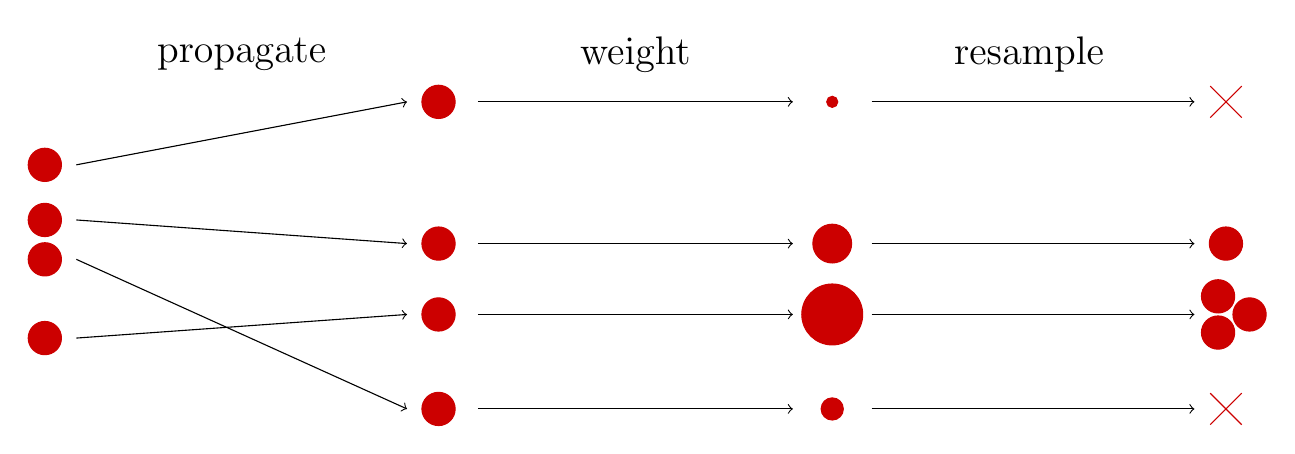
\begin{tikzpicture}
\filldraw[darkred] (0,0) circle (6pt);
\filldraw[darkred] (0,1) circle (6pt);
\filldraw[darkred] (0,1.5) circle (6pt);
\filldraw[darkred] (0,2.2) circle (6pt);

\draw[->] (0.4,2.2) -- (4.6,3);
\draw[->] (0.4,1.5) -- (4.6,1.2);
\draw[->] (0.4,1) -- (4.6,-0.9);
\draw[->] (0.4,0) -- (4.6,0.3);

\filldraw[darkred] (5,0.3) circle (6pt);
\filldraw[darkred] (5,-0.9) circle (6pt);
\filldraw[darkred] (5,1.2) circle (6pt);
\filldraw[darkred] (5,3) circle (6pt);

\draw[->] (5.5,3) -- (9.5,3);
\draw[->] (5.5,1.2) -- (9.5,1.2);
\draw[->] (5.5,-0.9) -- (9.5,-0.9);
\draw[->] (5.5,0.3) -- (9.5,0.3);

\filldraw[darkred] (10,0.3) circle (11pt);
\filldraw[darkred] (10,-0.9) circle (4pt);
\filldraw[darkred] (10,1.2) circle (7pt);
\filldraw[darkred] (10,3) circle (2pt);

\draw[->] (10.5,1.2) -- (14.6,1.2);
\draw[->] (10.5,0.3) -- (14.6,0.3);
\draw[->] (10.5,-0.9) -- (14.6,-0.9);
\draw[->] (10.5,3) -- (14.6,3);

\filldraw[darkred] (15.3,0.3) circle (6pt);
\filldraw[darkred] (14.9,0.53) circle (6pt);
\filldraw[darkred] (14.9,0.07) circle (6pt);
\filldraw[darkred] (15,1.2) circle (6pt);

\draw[darkred] (14.8,3.2) -- (15.2, 2.8);
\draw[darkred] (14.8,2.8) -- (15.2, 3.2);
\draw[darkred] (14.8,-0.7) -- (15.2, -1.1);
\draw[darkred] (14.8,-1.1) -- (15.2, -0.7);

\node at (2.5,3.6) {\Large{propagate}};
\node at (7.5,3.6) {\Large{weight}};
\node at (12.5,3.6) {\Large{resample}};
\end{tikzpicture}
}
\end{center}
\end{column}
\begin{column}{0.45\textwidth}
\textcolor{darkred}{Resampling induces a genealogy}\\
%% add tikz diagram of genealogy
We want to characterise the genealogies (in the limit as number of particles $N\to\infty$)
\end{column}
\end{columns}
\end{frame}

\begin{frame}
\begin{columns}
\begin{column}{0.45\textwidth}
\textcolor{darkred}{Kingman's coalescent} \\
Viewed backwards in time, genealogy becomes a coalescent
%% insert wiki pic of KC here
\end{column}
\begin{column}{0.45\textwidth}
\textcolor{darkred}{Results} \\
\begin{itemize}
\item foo
\end{itemize}
\end{column}
\end{columns}
\end{frame}


\end{document}